\documentclass[t,18pt]{beamer}
\usepackage[utf8]{inputenc}
\usepackage{graphbox}

\usetheme{Rochester}
\newcommand{\emdash}{---}

\setbeamercolor{normal text}{fg=black}
\setbeamercolor{frametitle}{fg=white}

\makeatletter
\setbeamertemplate{footline}
{
  \leavevmode%
  \hbox{%
  \begin{beamercolorbox}[wd=.5\paperwidth,ht=2.25ex,dp=1ex,center]{author in head/foot}%
    \usebeamerfont{author in head/foot}\insertshortauthor
  \end{beamercolorbox}%
  \begin{beamercolorbox}[wd=.5\paperwidth,ht=2.25ex,dp=1ex,right]{date in head/foot}%
    \usebeamerfont{date in head/foot}\insertshortdate{}\hspace*{2em}
    \insertframenumber{} / \inserttotalframenumber\hspace*{2ex}
  \end{beamercolorbox}}%
  \vskip0pt%
}
\makeatother





\begin{document}

\title{Visualizing Dynamic Clustered Data Using Area-proportional Maps}
\author{Christian Schnorr}

\begin{frame}
  \titlepage
\end{frame}

\begin{frame}
  \frametitle{Agenda}
  \begin{itemize}
    \item \nameref{sect:introduction}
    \item \nameref{sect:visualizing-static-input-graphs}
    \item \nameref{sect:visualizing-dynamic-input-graphs}
    \item \nameref{sect:evaluation}
  \end{itemize}
\end{frame}





\section{Introduction}
\label{sect:introduction}

\begin{frame}
  \frametitle{\nameref{sect:introduction}}
  \begin{itemize}
    \item \nameref{subsect:problem-statement}
    \item \nameref{subsect:motivation}
  \end{itemize}
\end{frame}

\subsection{Problem Statement}
\label{subsect:problem-statement}

\begin{frame}
  \frametitle{\nameref{subsect:problem-statement}}
  \begin{itemize}
    \item Visualize clustered graph as a map \begin{itemize}
      \item Each country represents a cluster in the original graph
      \item Countries have area close to proportional to cluster size
      \item Dynamic setting: input graph changes over time $\to$ map needs to adapt
    \end{itemize}
  \end{itemize}
\end{frame}

\subsection{Motivation}
\label{subsect:motivation}

\begin{frame}
  \frametitle{\nameref{subsect:motivation}}
  \begin{itemize}
    \item Clustered data appears naturally
    \item Map metaphor helps us make sense of data
    \item Dynamic data appears naturally: preserving mental map is crucial
    \item Area is a strong visual variable
    \item Motivating application: opinion networks
  \end{itemize}
\end{frame}





\section{Visualizing Static Input Graphs}
\label{sect:visualizing-static-input-graphs}

\begin{frame}
  \frametitle{\nameref{sect:visualizing-static-input-graphs}}
  \begin{itemize}
    \item \nameref{subsect:definitions}
    \item \nameref{subsect:algorithmic-pipeline-static}
    \item \nameref{subsect:requirements-on-input-graph}
    \item \nameref{subsect:transformation-to-dual}
    \item \nameref{subsect:drawing-the-polygonal-dual}
  \end{itemize}
\end{frame}

\subsection{Definitions}
\label{subsect:definitions}

\begin{frame}
  \frametitle{\nameref{subsect:definitions}}
  \begin{itemize}
    \item Polygonal contact representation \begin{itemize}
      \item Contact representation in which all regions are simple polygons
      \item No holes
      \item No duplicate adjacencies
    \end{itemize}
    \item Polygonal dual of graph G \begin{itemize}
      \item Polygonal contact representation of G
    \end{itemize}
  \end{itemize}
\end{frame}

\subsection{Algorithmic Pipeline}
\label{subsect:algorithmic-pipeline-static}

\begin{frame}[c]
  \frametitle{\nameref{subsect:algorithmic-pipeline-static}}
  \begin{figure}
    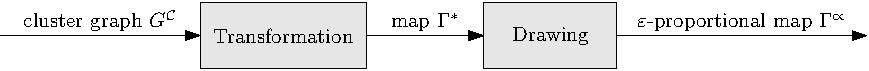
\includegraphics[width=\textwidth]{../Thesis/Resources/Framework-1.pdf}
  \end{figure}
\end{frame}

\subsection{Requirements on Input Graph}
\label{subsect:requirements-on-input-graph}

\begin{frame}
  \frametitle{\nameref{subsect:requirements-on-input-graph}}
  \begin{itemize}
    \item Plane
    \item Internally triangulated
    \item Biconnected
    \item Vertex-weighted
  \end{itemize}
\end{frame}

\subsection{Transformation to Dual}
\label{subsect:transformation-to-dual}

\begin{frame}[c]
  \frametitle{\nameref{subsect:transformation-to-dual}}
  \begin{figure}
    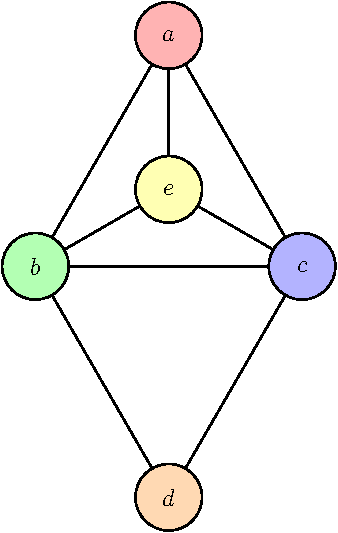
\includegraphics[align=c,height=2.90908cm]{../Thesis/Resources/Transformation-AugmentedDual-1.pdf}\;
    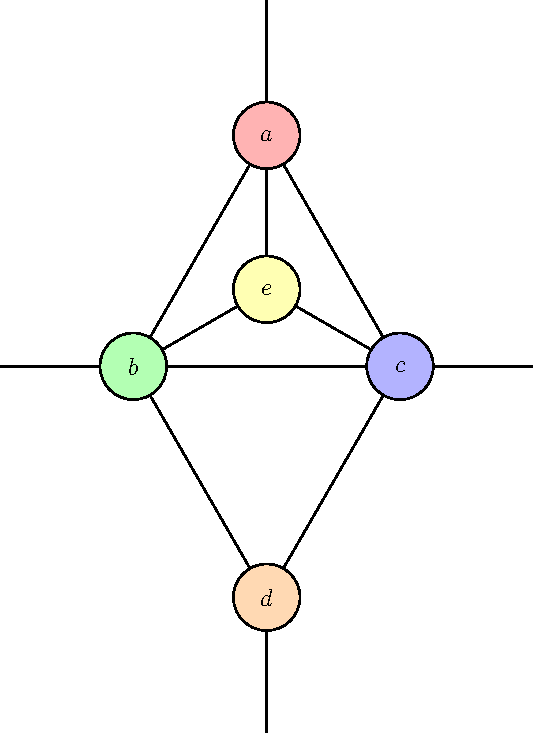
\includegraphics[align=c,height=4cm]{../Thesis/Resources/Transformation-AugmentedDual-2.pdf}\;
    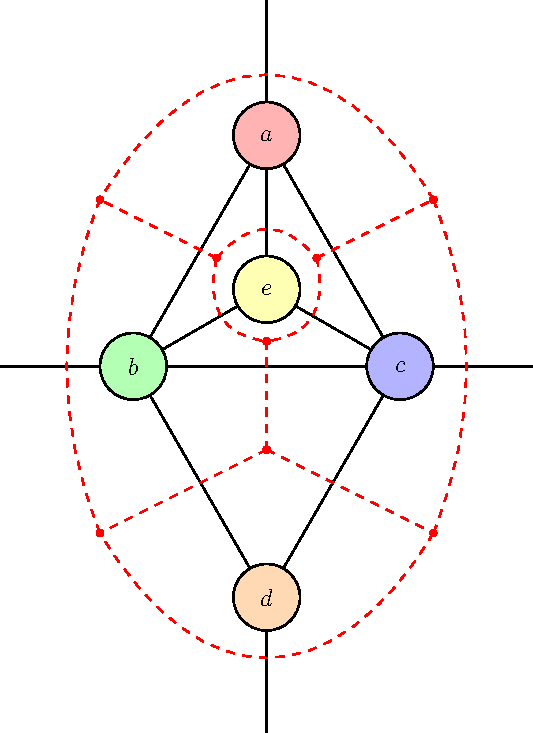
\includegraphics[align=c,height=4cm]{../Thesis/Resources/Transformation-AugmentedDual-3.pdf}\;
    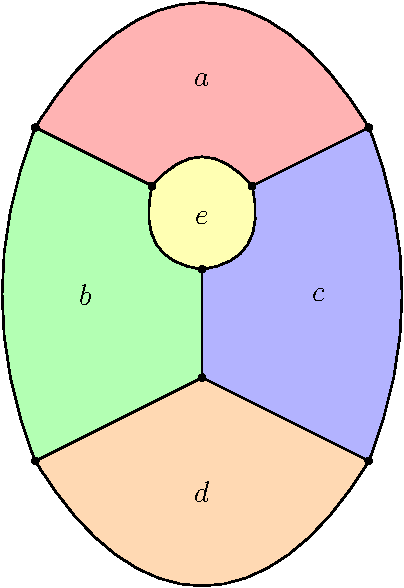
\includegraphics[align=c,height=3.5cm]{../Thesis/Resources/Transformation-AugmentedDual-4.pdf}
  \end{figure}
\end{frame}

\subsection{Drawing the Polygonal Dual}
\label{subsect:drawing-the-polygonal-dual}

\begin{frame}[c]
  \frametitle{\nameref{subsect:transformation-to-dual}}
  \begin{figure}
    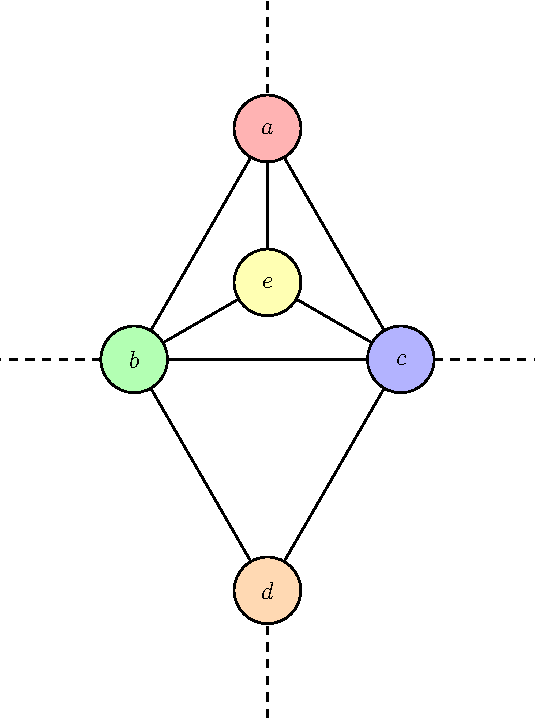
\includegraphics[align=c,height=5cm]{../Thesis/Resources/Transformation-Algorithm-2.pdf}\qquad
    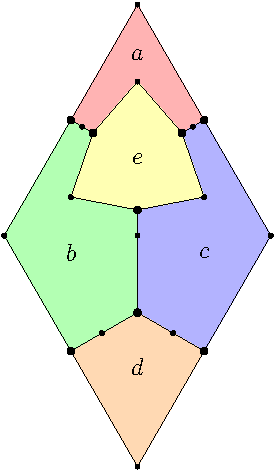
\includegraphics[align=c,height=3.2753cm]{../Thesis/Resources/Transformation-Algorithm-3.pdf}\qquad
    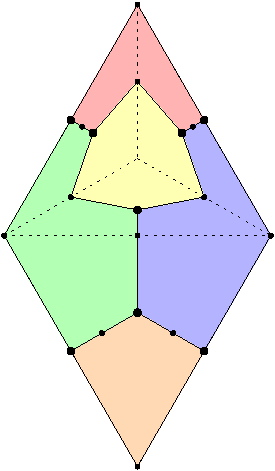
\includegraphics[align=c,height=3.2753cm]{../Thesis/Resources/Transformation-Algorithm-4.pdf}
  \end{figure}
\end{frame}

\begin{frame}
  \frametitle{\nameref{subsect:drawing-the-polygonal-dual}}
  \begin{itemize}
    \item Force-directed graph drawing \begin{itemize}
      \item Air pressure
      \item Angular resolution
      \item Vertex-vertex repulsion
      \item Vertex-edge repulsion
    \end{itemize}
    \item Preserve edge crossing and combinatorial properties: ImPrEd
  \end{itemize}
\end{frame}





\section{Visualizing Dynamic Input Graphs}
\label{sect:visualizing-dynamic-input-graphs}

\begin{frame}
  \frametitle{\nameref{sect:visualizing-dynamic-input-graphs}}
  \begin{itemize}
    \item \nameref{subsect:algorithmic-pipeline-dynamic}
    \item \nameref{subsect:incremental-transformation} \begin{itemize}
      \item \nameref{subsubsect:weight-changes}
      \item \nameref{subsubsect:inserting-vertices}
      \item \nameref{subsubsect:removing-vertices}
      \item \nameref{subsubsect:flipping-edges}
    \end{itemize}
  \end{itemize}
\end{frame}

\subsection{Algorithmic Pipeline}
\label{subsect:algorithmic-pipeline-dynamic}

\begin{frame}[c]
  \frametitle{\nameref{subsect:algorithmic-pipeline-static}}
  \begin{figure}
    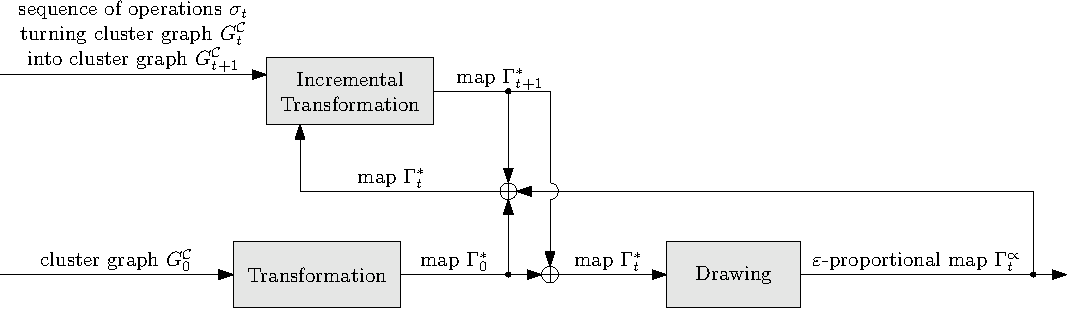
\includegraphics[width=\textwidth]{../Thesis/Resources/Framework-3.pdf}
  \end{figure}
\end{frame}

\subsection{Incremental Transformation}
\label{subsect:incremental-transformation}

\subsubsection{Weight Changes}
\label{subsubsect:weight-changes}

\subsubsection{Inserting Vertices}
\label{subsubsect:inserting-vertices}

\begin{frame}[c]
  \frametitle{\nameref{subsect:incremental-transformation}}
  \framesubtitle{Inserting Vertices Inside}
  \begin{figure}
    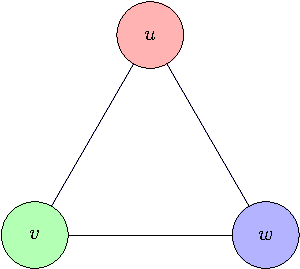
\includegraphics[height=2.5cm]{../Thesis/Resources/InsertVertex-Example-Inside-1.pdf}
    \quad
    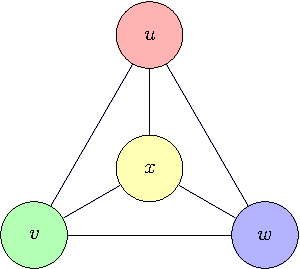
\includegraphics[height=2.5cm]{../Thesis/Resources/InsertVertex-Example-Inside-2.pdf}
  \end{figure}
  \begin{figure}
    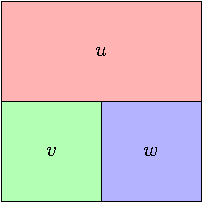
\includegraphics[height=2.5cm]{../Thesis/Resources/InsertVertex-Example-Inside-3.pdf}
    \qquad
    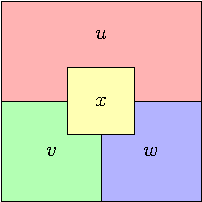
\includegraphics[height=2.5cm]{../Thesis/Resources/InsertVertex-Example-Inside-4.pdf}
  \end{figure}
\end{frame}

\begin{frame}
  \frametitle{\nameref{subsect:incremental-transformation}}
  \framesubtitle{Inserting Vertices Inside}
  \begin{itemize}
    \item Internal faces in primal are triangles
    \item No preconditions
    \vspace{1cm}
    \item<2-> Idea: insert new face in dual at point where three existing faces meet
  \end{itemize}
\end{frame}

\begin{frame}[c]
  \frametitle{\nameref{subsect:incremental-transformation}}
  \framesubtitle{Inserting Vertices Inside \emdash{} Illustration}
  \begin{figure}
    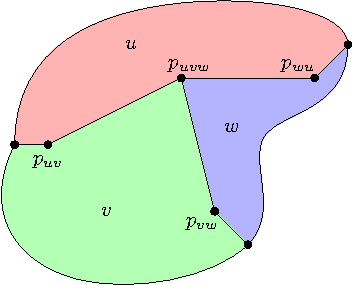
\includegraphics[height=2.7cm]{../Thesis/Resources/InsertVertex-Illustration-1.pdf}\quad
    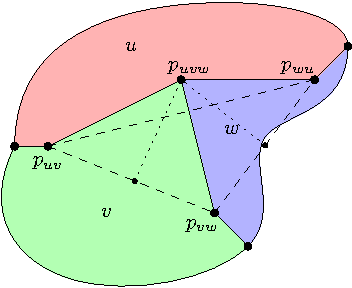
\includegraphics[height=2.7cm]{../Thesis/Resources/InsertVertex-Illustration-2.pdf}\quad
    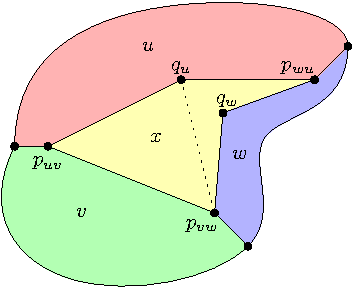
\includegraphics[height=2.7cm]{../Thesis/Resources/InsertVertex-Illustration-3.pdf}
  \end{figure}
\end{frame}

\begin{frame}[c]
  \frametitle{\nameref{subsect:incremental-transformation}}
  \framesubtitle{Inserting Vertices Outside}
  \begin{figure}
    \qquad
    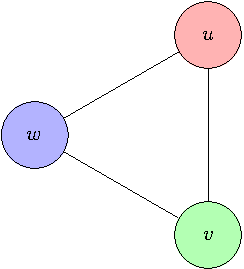
\includegraphics[height=2.5cm]{../Thesis/Resources/InsertVertex-Example-Outside-1.pdf}
    \quad
    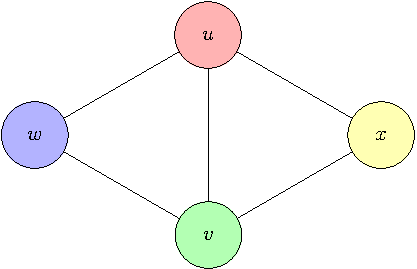
\includegraphics[height=2.5cm]{../Thesis/Resources/InsertVertex-Example-Outside-2.pdf}
  \end{figure}
  \begin{figure}
    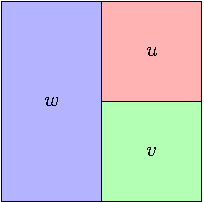
\includegraphics[height=2.5cm]{../Thesis/Resources/InsertVertex-Example-Outside-3.pdf}
    \qquad
    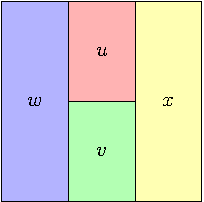
\includegraphics[height=2.5cm]{../Thesis/Resources/InsertVertex-Example-Outside-4.pdf}
  \end{figure}
\end{frame}

\begin{frame}
  \frametitle{\nameref{subsect:incremental-transformation}}
  \framesubtitle{Inserting Vertices Outside}
  \begin{itemize}
    \item Primal must remain biconnected and internally triangulated
    \item Neighbors must form a path on outer face
    \item Here: only add vertices to 2 adjacent vertices on outer face
    \vspace{1cm}
    \item<2-> Idea: same as vertex insertion inside
  \end{itemize}
\end{frame}

\begin{frame}[c]
  \frametitle{\nameref{subsect:incremental-transformation}}
  \framesubtitle{Inserting Vertices Outside \emdash{} Implicit Outer Face}
  \begin{figure}
    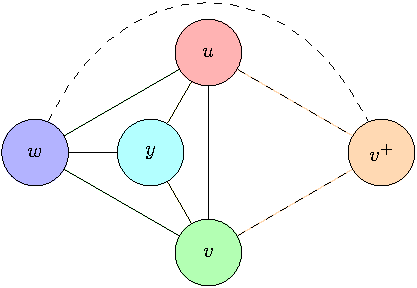
\includegraphics[height=2.5cm]{../Thesis/Resources/InsertVertex-Duality-1.pdf}
    \quad
    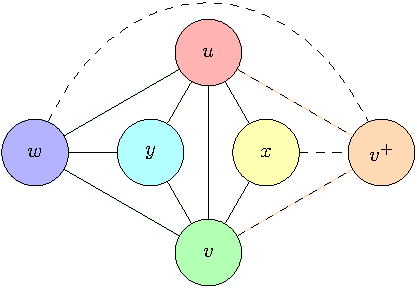
\includegraphics[height=2.5cm]{../Thesis/Resources/InsertVertex-Duality-2.pdf}
  \end{figure}
  \begin{figure}
    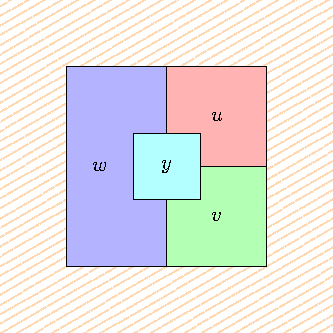
\includegraphics[height=2.5cm]{../Thesis/Resources/InsertVertex-Duality-3.pdf}
    \qquad\qquad
    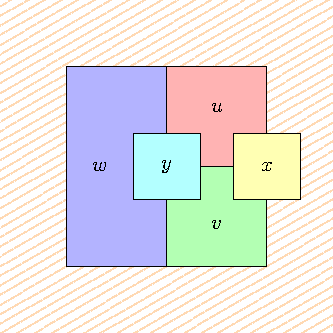
\includegraphics[height=2.5cm]{../Thesis/Resources/InsertVertex-Duality-4.pdf}
  \end{figure}
\end{frame}

\subsubsection{Removing Vertices}
\label{subsubsect:removing-vertices}

\begin{frame}[c]
  \frametitle{\nameref{subsect:incremental-transformation}}
  \framesubtitle{Removing Internal Vertices}
  \begin{figure}
    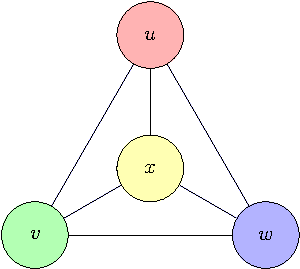
\includegraphics[height=2.5cm]{../Thesis/Resources/RemoveVertex-Example-Internal-1.pdf}
    \quad
    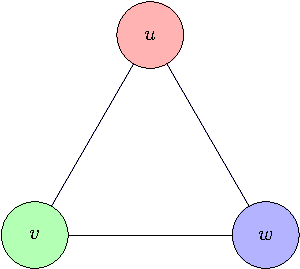
\includegraphics[height=2.5cm]{../Thesis/Resources/RemoveVertex-Example-Internal-2.pdf}
  \end{figure}
  \begin{figure}
    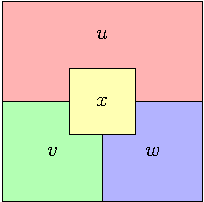
\includegraphics[height=2.5cm]{../Thesis/Resources/RemoveVertex-Example-Internal-3.pdf}
    \qquad
    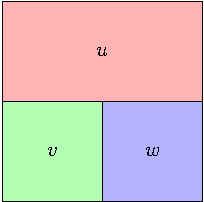
\includegraphics[height=2.5cm]{../Thesis/Resources/RemoveVertex-Example-Internal-4.pdf}
  \end{figure}
\end{frame}

\begin{frame}
  \frametitle{\nameref{subsect:incremental-transformation}}
  \framesubtitle{Removing Internal Vertices}
  \begin{itemize}
    \item Primal must remain internally triangulated
    \item Vertex to be removed must have degree 3
    \vspace{1cm}
    \item<2-> Idea: remove boundary with one adjacent region
  \end{itemize}
\end{frame}

\begin{frame}[c]
  \frametitle{\nameref{subsect:incremental-transformation}}
  \framesubtitle{Inserting Internal Vertices \emdash{} Illustration}
  \begin{figure}
    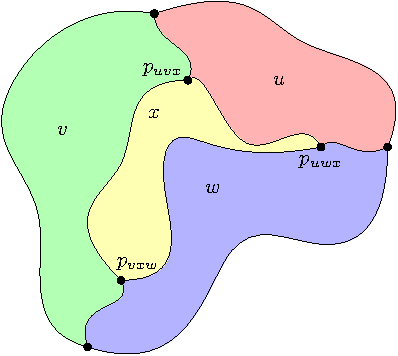
\includegraphics[height=4cm]{../Thesis/Resources/RemoveVertex-Illustration-1.pdf}
    \qquad
    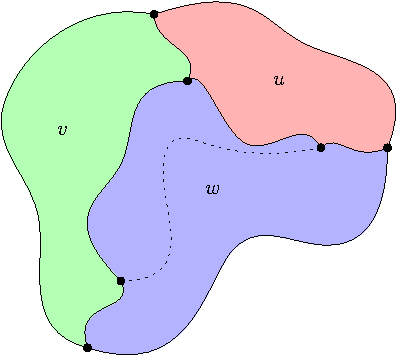
\includegraphics[height=4cm]{../Thesis/Resources/RemoveVertex-Illustration-2.pdf}
  \end{figure}
\end{frame}

\begin{frame}[c]
  \frametitle{\nameref{subsect:incremental-transformation}}
  \framesubtitle{Removing External Vertices}
  \begin{figure}
    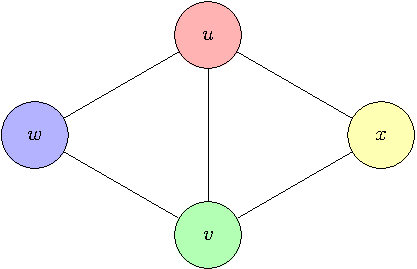
\includegraphics[height=2.5cm]{../Thesis/Resources/RemoveVertex-Example-External-1.pdf}
    \qquad
    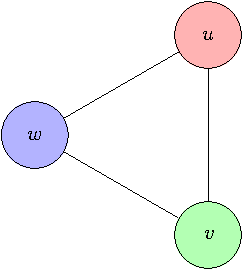
\includegraphics[height=2.5cm]{../Thesis/Resources/RemoveVertex-Example-External-2.pdf}
    \qquad\qquad
  \end{figure}
  \begin{figure}
    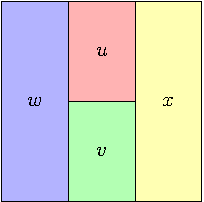
\includegraphics[height=2.5cm]{../Thesis/Resources/RemoveVertex-Example-External-3.pdf}
    \qquad\qquad
    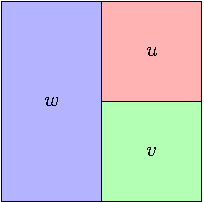
\includegraphics[height=2.5cm]{../Thesis/Resources/RemoveVertex-Example-External-4.pdf}
  \end{figure}
\end{frame}

\begin{frame}
  \frametitle{\nameref{subsect:incremental-transformation}}
  \framesubtitle{Removing External Vertices}
  \begin{itemize}
    \item Primal must remain biconnected
    \item Graph must have 4+ vertices beforehand
    \item Here: only vertices of degree 2
    \vspace{1cm}
    \item<2-> Idea: same as removing internal vertices
  \end{itemize}
\end{frame}

\subsubsection{Flipping Edges}
\label{subsubsect:flipping-edges}

\begin{frame}[c]
  \frametitle{\nameref{subsect:incremental-transformation}}
  \framesubtitle{Flipping Edges}
  \begin{figure}
    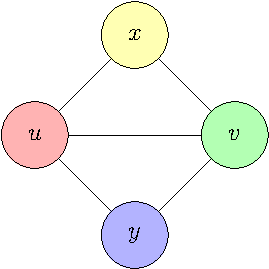
\includegraphics[height=2.5cm]{../Thesis/Resources/FlipEdge-Example-Internal-1.pdf}
    \quad
    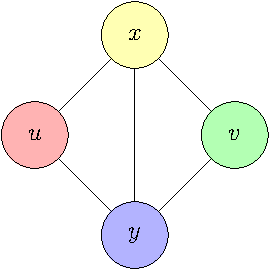
\includegraphics[height=2.5cm]{../Thesis/Resources/FlipEdge-Example-Internal-2.pdf}
  \end{figure}
  \begin{figure}
    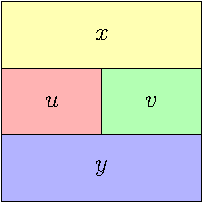
\includegraphics[height=2.5cm]{../Thesis/Resources/FlipEdge-Example-Internal-3.pdf}
    \qquad
    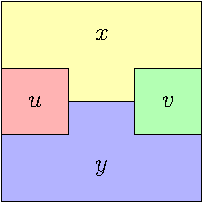
\includegraphics[height=2.5cm]{../Thesis/Resources/FlipEdge-Example-Internal-4.pdf}
  \end{figure}
\end{frame}

\begin{frame}
  \frametitle{\nameref{subsect:incremental-transformation}}
  \framesubtitle{Flipping Edges}
  \begin{itemize}
    \item Internal edge is incident to two triangular faces
    \item Edge can only be flipped if vertices on either side aren’t already adjacent
    \vspace{1cm}
    \item<2-> Idea \begin{itemize}
      \item<2-> Contact boundary to be removed into single point
      \item<2-> Create boundary in opposing direction
    \end{itemize}
  \end{itemize}
\end{frame}

\begin{frame}[c]
  \frametitle{\nameref{subsect:incremental-transformation}}
  \framesubtitle{Flipping Edges \emdash{} Contract $u$-$v$-Boundary}
  \begin{figure}
    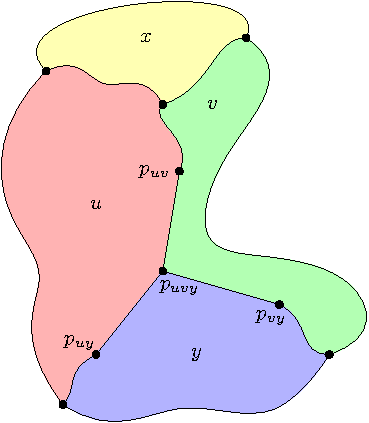
\includegraphics[width=3.25cm]{../Thesis/Resources/FlipEdge-ContractBoundaryBelow-1.pdf}
    \quad
    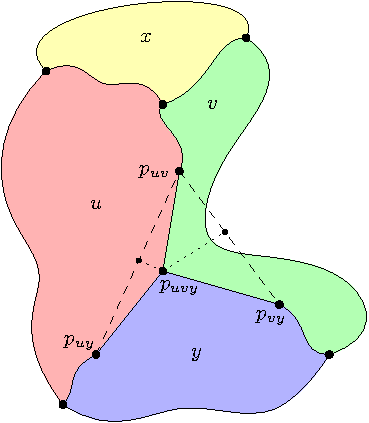
\includegraphics[width=3.25cm]{../Thesis/Resources/FlipEdge-ContractBoundaryBelow-2.pdf}
    \quad
    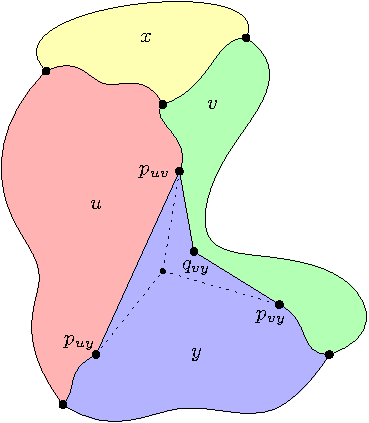
\includegraphics[width=3.25cm]{../Thesis/Resources/FlipEdge-ContractBoundaryBelow-3.pdf}
  \end{figure}
\end{frame}

\begin{frame}[c]
  \frametitle{\nameref{subsect:incremental-transformation}}
  \framesubtitle{Flipping Edges \emdash{} Contract $u$-$v$-Boundary}
  \begin{figure}
    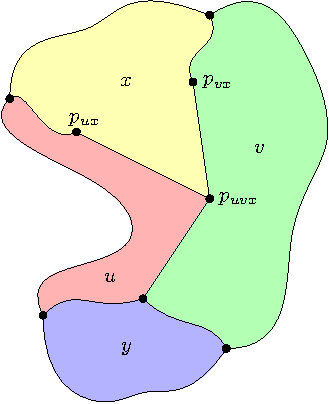
\includegraphics[width=3.25cm]{../Thesis/Resources/FlipEdge-ContractBoundaryAbove-1.pdf}
    \quad
    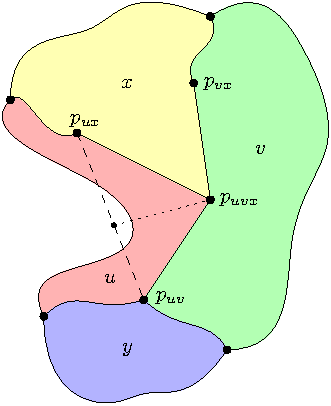
\includegraphics[width=3.25cm]{../Thesis/Resources/FlipEdge-ContractBoundaryAbove-2.pdf}
    \quad
    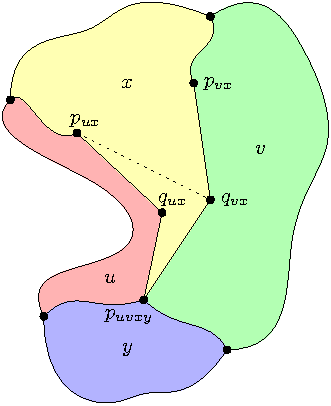
\includegraphics[width=3.25cm]{../Thesis/Resources/FlipEdge-ContractBoundaryAbove-3.pdf}
  \end{figure}
\end{frame}

\begin{frame}[c]
  \frametitle{\nameref{subsect:incremental-transformation}}
  \framesubtitle{Flipping Edges \emdash{} Create $x$-$y$-Boundary}
  \begin{figure}
    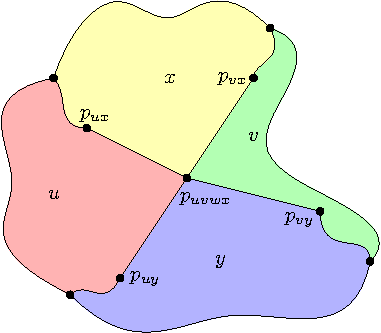
\includegraphics[width=3.25cm]{../Thesis/Resources/FlipEdge-StretchBoundary-1.pdf}
    \quad
    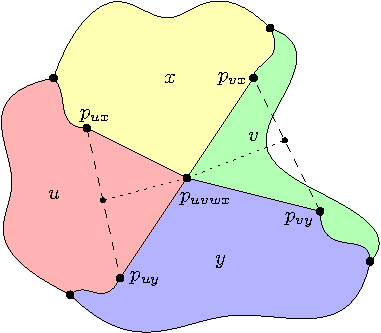
\includegraphics[width=3.25cm]{../Thesis/Resources/FlipEdge-StretchBoundary-2.pdf}
    \quad
    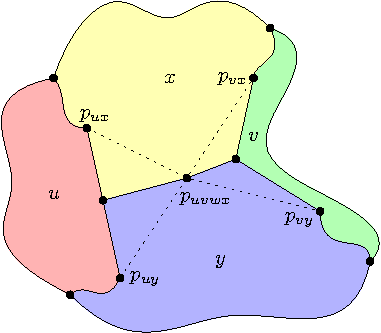
\includegraphics[width=3.25cm]{../Thesis/Resources/FlipEdge-StretchBoundary-3.pdf}
  \end{figure}
\end{frame}

\begin{frame}[c]
  \frametitle{\nameref{subsect:incremental-transformation}}
  \framesubtitle{Flipping Edges \emdash{} Inserting Edges into Outer Face}
  \begin{figure}
    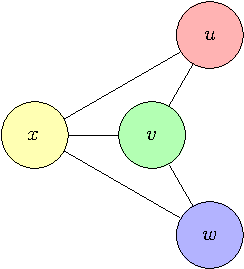
\includegraphics[height=2.5cm]{../Thesis/Resources/FlipEdge-Example-Insert-1.pdf}
    \qquad\quad
    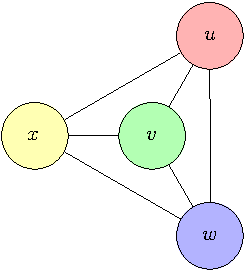
\includegraphics[height=2.5cm]{../Thesis/Resources/FlipEdge-Example-Insert-2.pdf}
  \end{figure}
  \begin{figure}
    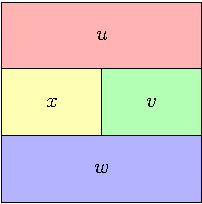
\includegraphics[height=2.5cm]{../Thesis/Resources/FlipEdge-Example-Insert-3.pdf}
    \qquad
    \includegraphics[height=2.5cm]{../Thesis/Resources/FlipEdge-Example-Insert-4.pdf}
  \end{figure}
\end{frame}

\begin{frame}[c]
  \frametitle{\nameref{subsect:incremental-transformation}}
  \framesubtitle{Flipping Edges \emdash{} Removing Edges from Outer Face}
  \begin{figure}
    \includegraphics[height=2.5cm]{../Thesis/Resources/FlipEdge-Example-Remove-1.pdf}
    \qquad\quad
    \includegraphics[height=2.5cm]{../Thesis/Resources/FlipEdge-Example-Remove-2.pdf}
  \end{figure}
  \begin{figure}
    \includegraphics[height=2.5cm]{../Thesis/Resources/FlipEdge-Example-Remove-3.pdf}
    \qquad
    \includegraphics[height=2.5cm]{../Thesis/Resources/FlipEdge-Example-Remove-4.pdf}
  \end{figure}
\end{frame}





\section{Evaluation}
\label{sect:evaluation}

\begin{frame}
  \frametitle{\nameref{sect:evaluation}}
  \begin{itemize}
    \item \nameref{subsect:research-questions}
    \item \nameref{subsect:quality-metrics}
    \item \nameref{subsect:test-case-generation}
    \item \nameref{subsect:evaluation-results}
    \item \nameref{subsect:examples}
  \end{itemize}
\end{frame}

\subsection{Research questions}
\label{subsect:research-questions}

\begin{frame}
  \frametitle{\nameref{subsect:research-questions}}
  \begin{enumerate}
    \item Which quantitative measures best capture the quality of the maps generated by our algorithm in terms of 
accuracy? \begin{itemize}
      \item our understanding of locally fat regions?
    \end{itemize}
    \item What is the quality of the maps generated by our algorithm according to these quality metrics? \begin{itemize}
      \item How does this quality change based on the size and other properties of the input graph? 
      \item How does this quality change over time as dynamic updates are incorporated? 
    \end{itemize}
  \end{enumerate}
\end{frame}

\subsection{Quality metrics}
\label{subsect:quality-metrics}

\begin{frame}
  \frametitle{\nameref{subsect:quality-metrics}}
  \begin{itemize}
    \item Normalized cartographic error \begin{itemize}
      \item Deviation of actual area from prescribed area
    \end{itemize}
    \item Polygon complexity \begin{itemize}
      \item Combination of frequency and amplitude of “vibration”of boundary and convexness of polygon
    \end{itemize}
    \vspace{1cm}
    \item Maximum and average values
  \end{itemize}
\end{frame}

\subsection{Test case generation}
\label{subsect:test-case-generation}

\begin{frame}
  \frametitle{\nameref{subsect:test-case-generation}}
  \framesubtitle{Parameters}
  \begin{itemize}
    \item Number of clusters $n$
    \item Bounding box $\mathcal{A} = \lbrack x_\text{min}, x_\text{max} \rbrack \times \lbrack y_\text{min}, y_\text{max} \rbrack$
    \item Weight distribution $\text{pmf} \colon \mathbb{N}_+ \to \mathbb{R}_+$
    \item Nesting ratio $\alpha$
    \item Nesting bias $\beta$
  \end{itemize}
\end{frame}

\begin{frame}
  \frametitle{\nameref{subsect:test-case-generation}}
  \framesubtitle{Algorithm Overview}
  \begin{itemize}
    \item Generate random vertex positions in bounding box
    \item Compute Delaunay triangulation
    \item Nest remaining vertices into existing triangular faces
    \item Sample weights according to weight distribution
    \item Sequence of dynamic operations is chosen at random	
  \end{itemize}
\end{frame}

\subsection{Evaluation Results}
\label{subsect:evaluation-results}

\begin{frame}[c]
  \frametitle{\nameref{subsect:evaluation-results}}
  \framesubtitle{Effect of initial number of clusters}
  \begin{figure}
    \includegraphics[width=5cm]{../Thesis/Resources/Evaluation-AverageCartographicError-n.pdf}
    \quad
    \includegraphics[width=5cm]{../Thesis/Resources/Evaluation-AveragePolygonComplexity-n.pdf}
  \end{figure}
\end{frame}

\begin{frame}[c]
  \frametitle{\nameref{subsect:evaluation-results}}
  \framesubtitle{Effect of number of operations}
  \begin{figure}
    \includegraphics[width=5cm]{../Thesis/Resources/Evaluation-AverageCartographicError-t.pdf}
    \quad
    \includegraphics[width=5cm]{../Thesis/Resources/Evaluation-AveragePolygonComplexity-t.pdf}
  \end{figure}
\end{frame}

\begin{frame}[c]
  \frametitle{\nameref{subsect:evaluation-results}}
  \framesubtitle{Effect of nesting ratio and bias}
  \begin{figure}
    \includegraphics[width=5cm]{../Thesis/Resources/Evaluation-AverageCartographicError-ab.pdf}
    \quad
    \includegraphics[width=5cm]{../Thesis/Resources/Evaluation-AveragePolygonComplexity-ab.pdf}
  \end{figure}
\end{frame}

\subsection{Examples}
\label{subsect:examples}

\begin{frame}[c]
  \frametitle{\nameref{subsect:examples}}
  \framesubtitle{Dynamics}
  \includegraphics[width=2.5cm]{../Thesis/Resources/Evaluation-Example-Dynamics-AE097F3A-14FD-4735-A19B-8FD343CA3346-0.pdf}
  \includegraphics[width=2.5cm]{../Thesis/Resources/Evaluation-Example-Dynamics-AE097F3A-14FD-4735-A19B-8FD343CA3346-1.pdf}
  \includegraphics[width=2.5cm]{../Thesis/Resources/Evaluation-Example-Dynamics-AE097F3A-14FD-4735-A19B-8FD343CA3346-2.pdf}
  \includegraphics[width=2.5cm]{../Thesis/Resources/Evaluation-Example-Dynamics-AE097F3A-14FD-4735-A19B-8FD343CA3346-3.pdf}
  \includegraphics[width=2.5cm]{../Thesis/Resources/Evaluation-Example-Dynamics-AE097F3A-14FD-4735-A19B-8FD343CA3346-0-P.pdf}
  \includegraphics[width=2.5cm]{../Thesis/Resources/Evaluation-Example-Dynamics-AE097F3A-14FD-4735-A19B-8FD343CA3346-1-P.pdf}
  \includegraphics[width=2.5cm]{../Thesis/Resources/Evaluation-Example-Dynamics-AE097F3A-14FD-4735-A19B-8FD343CA3346-2-P.pdf}
  \includegraphics[width=2.5cm]{../Thesis/Resources/Evaluation-Example-Dynamics-AE097F3A-14FD-4735-A19B-8FD343CA3346-3-P.pdf}
\end{frame}

\begin{frame}
  \frametitle{\nameref{subsect:examples}}
  \framesubtitle{Maps with $n$ = 10}
  \begin{figure}
    \includegraphics[width=5cm]{../Thesis/Resources/Evaluation-Example-n10-0F69CDD9-EAAD-4F81-934F-8BA98B1424F6-2.pdf}
    \quad
    \includegraphics[width=5cm]{../Thesis/Resources/Evaluation-Example-n10-9A841901-DFA0-4ECD-A758-87E1C8A1D0D0-0.pdf}
  \end{figure}
\end{frame}

\begin{frame}
  \frametitle{\nameref{subsect:examples}}
  \framesubtitle{Maps with $n$ = 20}
  \begin{figure}
    \includegraphics[width=5cm]{../Thesis/Resources/Evaluation-Example-n20-450053F2-5F0A-4CFE-8A08-92CC201A07B9-0.pdf}
    \quad
    \includegraphics[width=5cm]{../Thesis/Resources/Evaluation-Example-n20-AE097F3A-14FD-4735-A19B-8FD343CA3346-0.pdf}
  \end{figure}
\end{frame}

\begin{frame}
  \frametitle{\nameref{subsect:examples}}
  \framesubtitle{Maps with $n$ = 30}
  \begin{figure}
    \includegraphics[width=5cm]{../Thesis/Resources/Evaluation-Example-n30-9BA67779-50C2-483B-8E81-916125D5D3F7-0.pdf}
    \quad
    \includegraphics[width=5cm]{../Thesis/Resources/Evaluation-Example-n30-45D8EAD2-210C-4F04-8C7F-EA3E65484875-0.pdf}
  \end{figure}
\end{frame}





\end{document}
